\hypertarget{section-better-proof-tools}{%
\section{Section: Better proof tools}\label{section-better-proof-tools}}

\interlude*<left,leftskip=7cm,>[90]<Tribulations \textasciitilde\ Tooling>{Oh These\\Proof Tools}<Vive la Révolution! Against the Bourgeoisie of Proof Assistants!>




\begin{frame}{Symbolic Modeling of Rosenpass}
\hypertarget{analysis-usability-colorful-proverif-voice}{}
  \begin{columns}[c]
    \begin{column}{.5\linewidth}
     \rlap{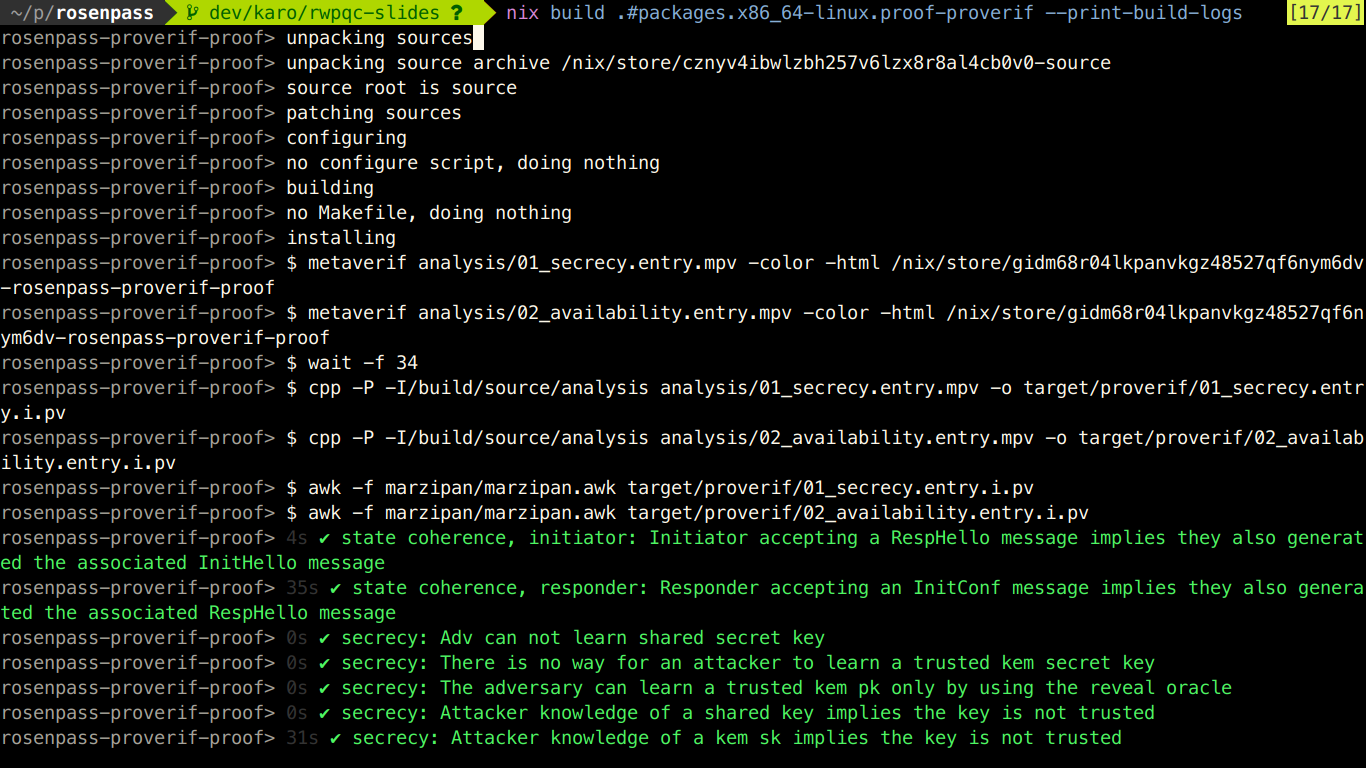
\includegraphics[keepaspectratio,height=.85\textheight]{graphics/2023-03-20-symbolic-analysis-screenshot.png}}
    \end{column}

	  %\pause

    \begin{column}{.5\linewidth}
    \tikz\node[rectangle,fill opacity=1,fill=white,minimum height=.85\textheight, text width=\linewidth]{
      \begin{itemize}
        \item Symbolic modeling using ProVerif
        \item Proofs treated as part of the codebase
        \item Uses a model internally that is based on a fairly comprehensive Maximum Exposure Attacks (MEX) variant
        \item Covers non-interruptability (resistance to disruption attacks)
        \item Mechanized proof in the computational model is an open issue
      \end{itemize}};
    \end{column}
  \end{columns}
\end{frame}




\begin{frame}{Problematic Parts of Pen-and-Paper Proofs}
\hypertarget{problematic-proofs}{}
  \begin{columns}[fullwidth,c]
    \begin{column}{.3\linewidth}
      
\includegraphics[width=\linewidth]{graphics/this-is-fine-crop.png}\\
      
\includegraphics[width=\linewidth]{graphics/this-is-not-fine-crop.jpg}%
    \end{column}
    \hspace{1.2em}
    \begin{column}{.68\linewidth}

      Bellare and Rogaway: [BR06]\\
      \hspace{1.618em} many “essentially unverifiable” proofs, “crisis of rigor”\\[1.5em]

      Halevi: [Hal05]\\
      \hspace{1.618em} some reasons are social, but “our proofs are truly complex”\\[1.5em]

      Joseph Jaeger: [ProTeCS 2024, Workshop at Eurocrypt]\\
      \hspace{1.618em} technical and social reasons\\
      \hspace{1.618em} why and for whom do we write proofs?\\[1.5em]%

      We'd like to add:\\
      \hspace{1.618em} pen-and-paper proofs are hard to maintain, update, reuse\\
      \hspace{1.618em} especially for 3rd parties\\[1.5em]%

      Can proofs become part of a continuous engineering effort?%
    \end{column}
  \end{columns}
\end{frame}
